%!TEX root = twig-language.tex

\section{Code generation}
\label{sec:code-gen}

To generate code, Twig relies on an abstract, language-independent model with a
small number of basic operations. This simplified model is useful for
formulating Twig's semantics, described in Section~\ref{sec:semantics}. It is
also helpful in clarifying the precise operations which Twig supports, without
getting bogged down in the (potentially complicated) details of outputting code
for a particular programming language.

Twig generates code in units called \emph{blocks}. The term ``block'' is
somewhat overloaded -- our usage differs from the norm. In Twig, a block of code
represents anything that performs some operation on a set of inputs, and which
produces a set of outputs. Blocks may have zero or more inputs and outputs. See
Figure~\ref{fig:blocks} for a visual representation. Blocks can also be combined
in two different ways: \emph{sequentially}, or \emph{in parallel}. These
operations are described in more detail below.

\begin{figure}[ht]
\centering
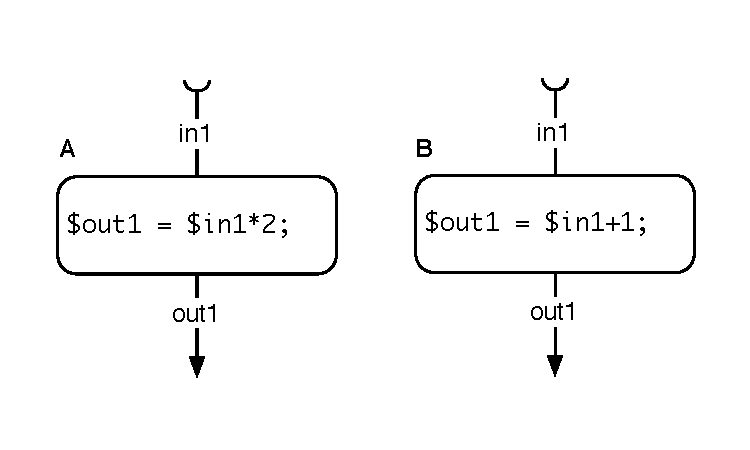
\includegraphics[width=0.75\columnwidth]{images/code-gen1}
\caption{Two basic blocks, A and B. Inputs are on top, outputs on the bottom.}
\label{fig:blocks}
\end{figure}

\subsection{Block Composition}

As mentioned above, Twig provides two fundamental binary operations on blocks.
The first is the \emph{sequential composition} operator, represented by the
addition symbol ($+$). Sequencing connects two blocks of code by ``wiring'' the
outputs of the first block into the inputs of the second. In C, this is done by
creating temporary variables which are substituted into the original blocks. For
example, see Figure~\ref{fig:codegen-seq}, which builds on
Figure~\ref{fig:blocks}.

\begin{figure}[ht]
\centering
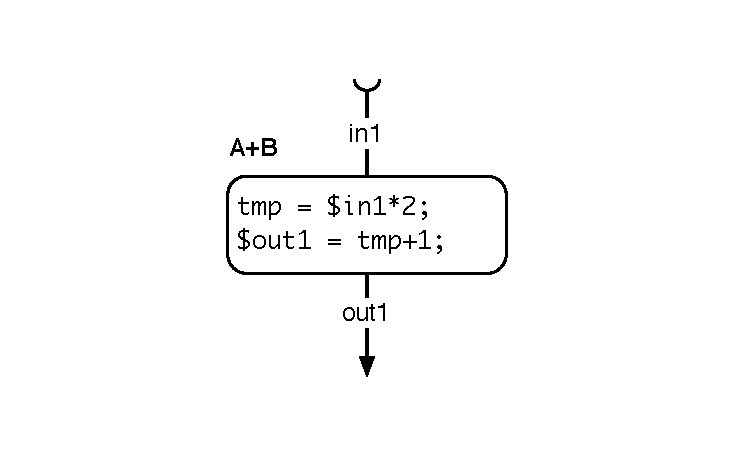
\includegraphics[width=0.75\columnwidth]{images/code-gen2}
\caption{Two blocks from Figure~\ref{fig:blocks} composed sequentially.
The variable ``tmp'' is created, and renaming performed, so that the output of
block A would flow to the input of block B.}
\label{fig:codegen-seq}
\end{figure}

Twig's implementation takes care of declaring and uniquely naming
temporary variables to accomplish sequencing.

The second operator is \emph{parallel composition}. Under this operator, two
blocks are combined so as to execute independently of one another, but to appear
as one single block. We represent this operation with the multiplication
operator ($\times$). An example is shown in Figure~\ref{fig:codegen-par}.

\begin{figure}[ht]
\centering
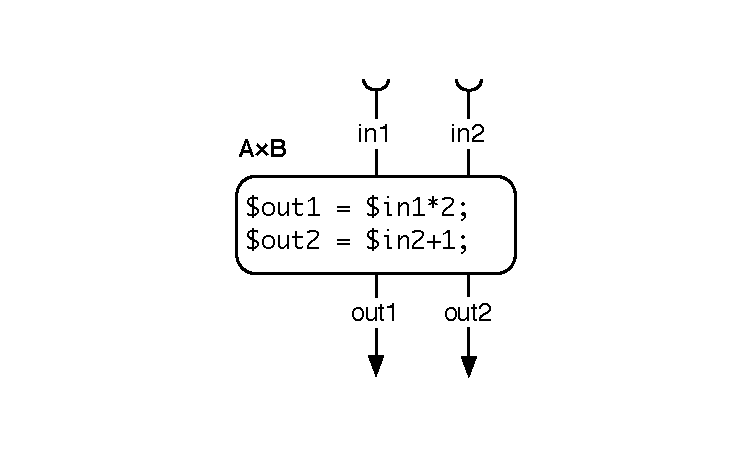
\includegraphics[width=0.75\columnwidth]{images/code-gen3}
\caption{Two blocks from Figure~\ref{fig:blocks} composed in parallel.
Renaming is performed such that the composed block has two inputs and two 
outputs.}
\label{fig:codegen-par}
\end{figure}

\subsection{Special Blocks}

Twig defines a special set of blocks called \emph{permutation} blocks. These
blocks have some special properties, which we will exploit for the purposes of
rewriting programs to remove redundant memory copies. In particular, some kinds
of blocks act as a kind of identity element when composed with others.

The permutation blocks are referred to as $\Pi_m(i_1,\ldots,i_n)$, and represent
the primitive operation of rearranging $m$ inputs to $n$ outputs, possibly in a
different order, and possibly duplicating or dropping elements. The data is only
passed through, and are otherwise unchanged.

Among the permutation blocks, there are a set of elements for which we provide
special rules; namely, a set of \emph{identity} permutations. The simplest of
these is $\Pi_1(1)$, which acts as an identity transformation with one input and
one output. We refer to this element as $I_1$. In fact, there are an unlimited
number of identity transformations, which take $n$ inputs to $n$ outputs,
unchanged. These are referred to as $I_n$, where $1 \leq n$, and $I_n =
\Pi_n(1,2,\ldots,n)$. The blocks $I_n$ are left- and right-identity elements
under a sequence operation. We sometimes use $I_n$ as a kind of ``no-op.''

Using this simple system, a wide variety of code can be generated.

% For all $x$ in $M$, we define two functions \texttt{in} and \texttt{out},
% which map elements in $M$ to, respectively, the number of inputs and outputs
% of the element. In either case, the number may be zero.
% 
% Given this structure, we provide two fundamental operations. The first is
% \emph{sequential composition}, where the outputs of one code block are fed
% into the inputs of another. We represent this operation as addition ($+$) and
% say that
% 
% \[
% \infer
% {x+y \in M}
% {x \in M \quad y \in M \quad \mathtt{out}(x) = \mathtt{in}(y)} \]
% 
% and
% 
% \begin{eqnarray*}
% \mathtt{in} (x+y) &=& \mathtt{in}(x)\\
% \mathtt{out}(x+y) &=& \mathtt{out}(y)
% \end{eqnarray*}
% 
% Note that the condition that the number of outputs on the left side equal the
% number of inputs on the right implies that $M$ is not closed under sequential
% composition. We take care in the design of the rest of Twig's semantics to
% ensure that this is never a problem.
% 
% The second operation is \emph{parallel composition}, where two blocks execute
% independently of one another. We represent this operation as multiplication
% ($\times$) and say that
% 
% \[
% \infer
% {x \times y \in M}
% {x \in M \quad y \in M}
% \]
% 
% and we define
% 
% \begin{eqnarray*}
% \mathtt{in} (x \times y) =& \mathtt{in}(x)  + \mathtt{in}(y)\\ \mathtt{out}(x
% \times y) =& \mathtt{out}(x) + \mathtt{out}(y) \end{eqnarray*}
% 
% Note that $M$ is closed under parallel composition.
% 
% We define a set of special elements in $M$, namely $\Pi_m(i_1,\ldots,i_n)$,
% where $i_1,\ldots,i_n \in \lbrace i | 1 \leq i \leq m \rbrace$. These are
% called \emph{permutation} elements, and represent the primitive operation of
% rearranging $m$ inputs to $n$ outputs, possibly in a different order, and
% possibly duplicating or dropping elements. The elements are only passed
% through, and are otherwise unchanged.
% 
% Among the permutation elements, there are a set of elements for which we
% provide special rules; namely, a set of \emph{identity} permutations. The
% simplest of these is $\Pi_1(1)$, which acts as an identity transformation with
% one input and one output. We refer to this element as $I_1$. In fact, there
% are an unlimited number of identity transformations, which take $n$ inputs to
% $n$ outputs, unchanged. These are referred to as $I_n$, where $1 \leq n$, and
% $I_n = \Pi_n(1,2,\ldots,n)$. Clearly,
% 
% \[
% \mathtt{in}(I_n) = \mathtt{out}(I_n) = n
% \]
% 
% Since the elements $I_n$ are intended to represent identity operations, we
% assign them a special meaning. Namely,
% 
% \[
% \infer{x + I_n \to x}{\mathtt{out}(x) = n} 
% \qquad
% \infer{I_n + x \to x}{\mathtt{in}(x) = n}
% \]
% 
% That is, $I_n$ acts as both a left- and right-identity when sequenced with a
% block $x$. We sometimes use $I_n$ as a kind of ``no-op.''
% 
% It is worth noting one further identity, namely
% 
% \[
% I_n = (I_1)^n
% \]
% 
% That is, $I_n$ is equivalent to the $n$-way parallel composition of $I_1$.
% 
% When $n$ is implied from the context we will sometimes write $I$ for $I_n$.
% For example, $x+I$ as a shorthand to refer to $x+I_n$ where $n =
% \mathtt{out}(x)$.
% 
% Using this simple system for composition, a wide variety of code can be
% generated.
